\section{Ziel}
\label{sec:Ziel}
Im laufe dieses Versuches soll das magnetische Moment eines Permanentmagneten durch zwei unterschiedliche Methoden bestimmt werden. Die Methoden sollen danach verglichen werden.

\section{Theorie}
\label{sec:Theorie}
Die grundlegenste Form des Magnetismus ist des Magnetismus ist der magnetische Dipol. Es gibt keine magnetischen Monopole. Da Monopole immer Quellen oder senken für Feldlinien sind
müssen Magnetfeldlinien immer geschlossen sein. Zur Untersuchung von Dipolen eignen sich Permanentmagneten oder eine geschlossene stromdurchflossene Leiterschleife, da diese sich 
wie mikroskopische magnetische Dipole verhalten. Das magnetische Moment $\vec{\mu}_{\text{Dipol}}$ ist eine wichtige Größe in der Magnetostatik und der Elektrodynamik, dass die stärke eines 
magnetischen Dipols beschreibt. Das magnetische Moment einer stromdurchflossenen Leiterschleife kann durch 
\begin{equation}
\label{eqn:mu Leiterschleife}
    \vec{\mu} = I \cdot \vec{A}
\end{equation}
berechnet werden, wobei $I$ der Strom und $\vec{A}$ die Querschnittsfläche der Leiterschleife ist. 


Das magnetische Moment eines Permanentmagneten kann nur experimentell bestimmt
werden. Dazu wird häufig eine makroskopischer magnetischer Dipol in einem homogenen Magnetfeld betrachtet. Befindet sich ein Dipol im Magnetfeld, so wirkt dieses ein Drehmoment
auf den Dipol. Dieses Drehmoment richtet den Dipol parallel zu den Feldlinien aus. Im homogenen Magnetfeld $\vec{B}$ wirkt ein Drehmoment $\vec{D}_{\text{B}}$: 
\begin{equation}
    \label{eqn:Drehmoment B-Feld}
    \vec{D}_{\text{B}} = \vec{\mu}_{\text{Dipol}} \times \vec{B}
\end{equation}
Dazu wirkt auch immer, wenn ein Drehbares Objekt nicht parallel zum Schwerefeld $\vv{F}_{\text{G}}$ ausgerichtet ist, ein Drehmoment $\vec{D}_{\text{G}}$ 
\begin{equation}
    \label{eqn:Drehmoment Schwerefeld}
    \vec{D}_{\text{G}} = m(\vv{r} \times \vv{g})
\end{equation}
auf das Objekt. Falls sich ein Gleichgewicht zwischen diesen Drehmomenten einstellt ergibt sich die Formel:

    
\begin{align*}
    \label{eqn:Drehmoment_Gleichgewicht}
    \vec{D}_{\text{B}} &= \vec{D}_{\text{G}} \\
    \Leftrightarrow \vec{\mu}_{\text{Dipol}} \times \vec{B} &= m(\vv{r} \times \vv{g})
\end{align*}

Man kann das Kreuzprodukt dann mit der allgemeinen Formel 
\begin{equation}
    \label{eqn:Kreuzprodukt}
    \vec{A} \times \vec{B} = \sin(\sphericalangle(\vec{A},\vec{B}))\lvert A \rvert \cdot\lvert B \rvert
\end{equation}
umschreiben. Dann erhält man
\begin{equation}
    \label{eqn:Drehmoment_Gleichgewicht1}
    \mu_{\text{Dipol}}\cdot B\cdot \sin\theta = m\cdot r\cdot g\cdot\sin\theta
\end{equation}
Nach kürzen von $\sin\theta$ und umstellen auf $\mu_{\text{Dipol}}$ erhält man schließlich den Ausdruck
\begin{equation}
    \label{eqn:Drehmoment_Gleichgewicht2}
    \mu_{\text{Dipol}} = \frac{m \cdot r\cdot g}{B} 
\end{equation}


Homogene Magnetfelder kommen nie natürlich vor. Aber man kann möglichst homogene Felder konstruieren. Dies kann durch ein Helmholtzspulenpaar realisiert werden.
\begin{figure}
	\centering
    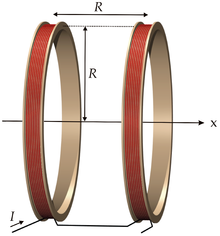
\includegraphics[width=0.4\textwidth]{content/Helmholtz_coils.png}
	\caption{Skizze eines Helmholtzspulenpaares \cite{Helmholtzspulenpaar}.}
	\label{fig:Helmholtzspulenpaar}
\end{figure}
Druch den Aufbau aus \autoref{fig:Helmholtzspulenpaar} bildet sich in der Mitte zwischen den beiden Spulen ein homogenes Magnetfeld entlang der Symetrieachse, welches 
nach außen inhomogener wird. Die Spulen müssen gleichsinnig vom Strom durchlaufen werden und der Radius der Spulen muss dem Abstand der beiden Spulen entsprechen. Das Magnetfeld
entlang der Symetrieachse für eine Spule mit einer Windung durch das Biot-Savart-Gesetz
\begin{equation}
    \label{eqn:diff_Biot-Savart}
    d\vv{B} = \frac{\mu_0 I}{4\pi}\frac{d\vec{s}\times\vec{r}}{r^3}
\end{equation}
nach Integration durch
\begin{equation}
    \label{eqn:Biot-Savart_1}
    \vv{B}(x) = \frac{\mu_0 I}{2}\frac{R^2}{\left(R^2 + x^2 \right)^{(3/2)}}\cdot \vec{e}_x
\end{equation}
berechnet werden. Hierbei wir die Symetrieachse als x-Achse definiert(vgl. \autoref{Helmholtzspulenpaar1}). Das "x" entspricht hier dem halben Abstand der beiden Spulen. 
\begin{figure}
	\centering
    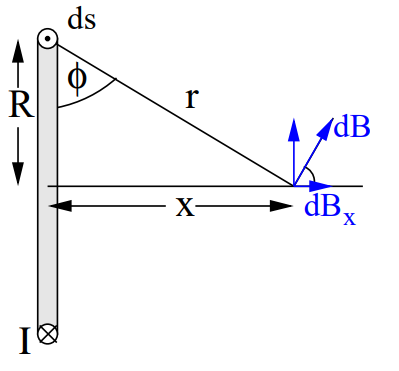
\includegraphics[width=0.4\textwidth]{content/Helmholtzachsen.PNG}
	\caption{Ergänzungsskizze der Achsen zum Helmholtzspulenpaares  \cite{v105}.}
	\label{fig:Helmholtzspulenpaar1}
\end{figure}
Das Magnetfeld im inneren des Helmholtzspulenpaares lässt sich nun durch Überlagerung der Einzelfelder bestimmen. Der Ursprung der gewählten Koordinaten wird dafür in die Mitte 
gesetzt und es werden pro Spule $N$ Windungen betrachtet. Daher ergibt sich das Magnetfeld an dieser Stelle zu
\begin{equation}
    \label{eqn:Helmholtz_B}
    B(0) = N\cdot B(-x) +N\cdot B(x) = \frac{N\mu_0 IR^2}{\left(R^2 + x^2 \right)^{(3/2)}}
\end{equation}


Eine weitere Methode zur Bestimmung des magnetischen Moments $\vv{\mu}_Dipol$ besteht durch Messung Schwingungsdauer eines Dipols, welcher im homogenen Magnetfeld
in Schwingung versetzt wird. Da sich ein schwingender Dipol im homogenen Magnetfeld wie ein harmonische Oszillator verhält, kann man dessen Bewegung beschreiben durch
\begin{equation}
    \label{eqn:BewegungsgleichungKugel}
    -\lvert \vv{\mu}_{\text{Dipol}} \times \vv{B}\rvert = J_{\text{K}} \cdot \frac{d^2 \theta}{dt^2}
\end{equation}
Diese Differenzialgelichung zweiter Ordnung hat eine Lösung durch die Schwin $T$. $T$ ist dabei bestimmt durch
\begin{equation}
    \label{eqn:Schwingungsdauer}
    T^2 = \frac{4{\pi}^2 J_{\text{K}}}{\vv{\mu}_{\text{Dipol}}}\frac{1}{B}
\end{equation} 
$J_{\text{K}}$ beschreibt hier ein Trägheitsmoment. Das Trägheitsmoment beschreibt die Trägheit eines rotierenden Körpers gegenüber der Änderung seiner Winkelgeschwindigkeit.
Allgemein gilt für das Trägheitsmoment $J$ die Formel:
\begin{equation}
    \label{eqn:Trägheitsmoment}
    J = \int_{\text{V}} {r^2}_{\bot} \text{d}m = \int_{\text{V}} {r^2}_{\bot} \rho \text{d}V
\end{equation} 
\cite{Demtröder_Exp_P_1}
Für den Spezialfall einer Kugel ergibt sich diese Formel zu:
\begin{equation}
    \label{eqn:Trägheitsmoment_Kugel}
    J_{\text{K}} = \frac{2}{5} m R^2
\end{equation}


